\documentclass[11pt,a4paper]{article}
\usepackage[top=19mm,bottom=18mm,left=20mm,right=20mm]{geometry}
\usepackage[T1]{fontenc}
\usepackage{lmodern}
\usepackage{booktabs}
\usepackage{graphicx}
\usepackage{float}
\usepackage{xcolor}
\usepackage{hyperref}

\definecolor{courseblue}{HTML}{004791}
\hypersetup{colorlinks=true,linkcolor=courseblue,urlcolor=courseblue,
  pdftitle={Assignment 2, Question 3 - Accelerate Llama2 Inference}}
\setlength{\parindent}{0pt}
\setlength{\parskip}{5pt}
\renewcommand{\arraystretch}{1.08}

\begin{document}
{\small\color{courseblue}Applied GPU Programming \enspace\textbullet\enspace Assignment 2, Question 3}\par
{\LARGE\bfseries Accelerate Llama2 Inference}\par
\smallskip

\section{Setup and implementation}

The experiment ran in Google Colab on an NVIDIA Tesla T4 with CUDA Toolkit
13.0.88 and Nsight Systems 2025.3.1. The baseline used Karpathy's FP32
\texttt{run.c} compiled with \texttt{gcc -O3} and the \texttt{stories15M.bin}
checkpoint. The matched benchmarks used greedy decoding (\texttt{-t 0}),
seed 42, an empty prompt, and a limit of 256 forward passes.

Each call to \texttt{matmul} multiplies a $d\times n$ weight matrix by a
length-$n$ input vector. One CUDA thread computes one output row, with
128 threads per block. The naive port allocates three device buffers,
copies the weights and input to the GPU, and copies the output back before
freeing the buffers. The optimized port uploads the checkpoint once,
locates each matrix by its offset in that copy, and reuses the input and
output buffers. Both ports use the same kernel.

\section{Correctness and throughput}

The three matched runs produced identical text. With \texttt{CHECK\_MATMUL=1},
both CUDA builds also passed an element-by-element CPU comparison for every
matmul in runs capped at eight steps. For a CPU result $y$, the allowed absolute
error was $10^{-5}+10^{-5}|y|$. CUDA compilation used \texttt{--fmad=false}
to keep multiplication and addition separate.

The instrumented CPU run counted \textbf{9,546 matmul calls} in the matched
workload. Each forward pass has seven projections in each of six layers
and one vocabulary projection, for $7\times6+1=43$ calls. The count
corresponds to 222 forward passes, with generation ending before the
256-step limit.

\begin{center}
\begin{tabular}{@{}lrr@{}}
\toprule
Run & Achieved tok/s & Relative to matched CPU \\
\midrule
CPU, README command & 43.416167 & --- \\
CPU, matched workload & 45.926850 & $1.00\times$ \\
Naive CUDA & 34.661230 & $0.75\times$ \\
Optimized CUDA & 283.697047 & $6.18\times$ \\
\bottomrule
\end{tabular}
\end{center}

Appendix~\ref{sec:run-screenshots} shows the original notebook screenshots
for the CPU README run and both CUDA runs.

\newpage
\section{Nsight Systems profiling}

We profiled the naive and optimized versions with the matched workload.
The traces cover initialization and generation. The inference program's
throughput timer starts after the first forward pass, so the throughput
in the previous section uses the unprofiled runs and excludes the
optimized version's one-time checkpoint upload.

\begin{center}
\begin{tabular}{@{}lrr@{}}
\toprule
Metric & Naive CUDA & Optimized CUDA \\
\midrule
\multicolumn{3}{@{}l}{\textbf{CUDA Runtime API}} \\
\texttt{cudaMalloc} calls & 28,638 & 3 \\
\texttt{cudaMalloc} total (ms) & 1,182.28 & 184.77 \\
\texttt{cudaFree} calls & 28,638 & 3 \\
\texttt{cudaFree} total (ms) & 965.91 & 0.34 \\
\texttt{cudaMemcpy} calls & 28,638 & 19,093 \\
\texttt{cudaMemcpy} total (ms) & 4,600.70 & 725.04 \\
\addlinespace
\multicolumn{3}{@{}l}{\textbf{GPU memory copies and kernel}} \\
Host-to-device copies & 19,092 & 9,547 \\
Host-to-device data (MB) & 13,500.470 & 74.370 \\
Host-to-device total (ms) & 2,306.40 & 20.46 \\
Device-to-host copies & 9,546 & 9,546 \\
Device-to-host data (MB) & 44.272 & 44.272 \\
Device-to-host total (ms) & 18.87 & 15.42 \\
\texttt{matvec\_kernel} launches & 9,546 & 9,546 \\
\texttt{matvec\_kernel} total (ms) & 492.22 & 523.64 \\
\bottomrule
\end{tabular}
\end{center}

\subsection*{Naive bottleneck}

\texttt{cudaMemcpy} accounted for 66.7\% of the recorded CUDA API time.
Allocation and release accounted for another 31.1\%. On the device,
host-to-device transfers took 2,306.40\,ms, compared with 492.22\,ms
for the matmul kernel. Each call uploaded its weight matrix again.
CUDA API times include host waiting during blocking operations and are
reported separately from GPU activity times.

\subsection*{Effect of persistent device buffers}

The optimized build issued 9,546 input uploads and one checkpoint
upload. Host-to-device volume fell by about $182\times$, and time in these
transfers fell by about $113\times$. The number of allocations and frees dropped
from three of each per matmul to three of each for the entire run.
Both versions launched 9,546 kernels and returned the same amount of
output data to the CPU. Total kernel time rose from 492.22 to 523.64\,ms
in the two captures. The optimized run reached \textbf{$8.18\times$ the
naive CUDA throughput} and \textbf{$6.18\times$ the matched CPU throughput}.

\medskip
{\small Measurements come from the saved outputs in \texttt{hw2\_Q3.ipynb}.
The implementation and build instructions are in \texttt{matmul\_cuda.cu},
\texttt{matmul\_cuda.h}, \texttt{run.patch}, and \texttt{Makefile}.
\href{https://github.com/karpathy/llama2.c/tree/350e04fe35433e6d2941dce5a1f53308f87058eb}{Upstream source}\enspace
\href{https://docs.nvidia.com/nsight-systems/AnalysisGuide/index.html}{Nsight Systems report guide}}

\newpage
\appendix
\section{Original benchmark screenshots}
\label{sec:run-screenshots}

The screenshots show the executed cells and their \texttt{achieved tok/s}
output in \texttt{hw2\_Q3.ipynb}.

\begin{figure}[H]
  \centering
  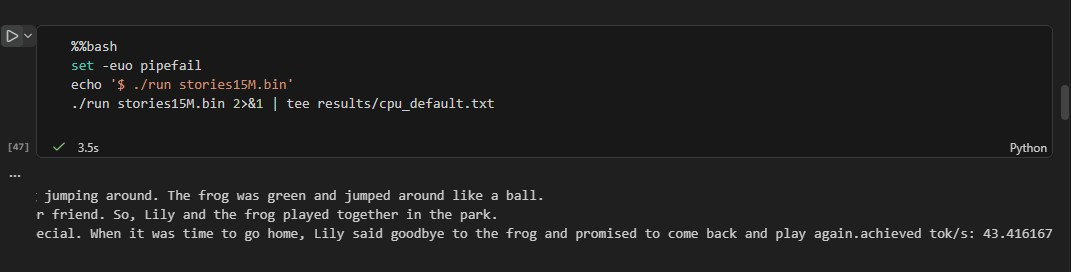
\includegraphics[width=\linewidth]{report_figures/47.jpg}
  \caption{Original CPU backend, README command (execution 47).}
\end{figure}

\begin{figure}[H]
  \centering
  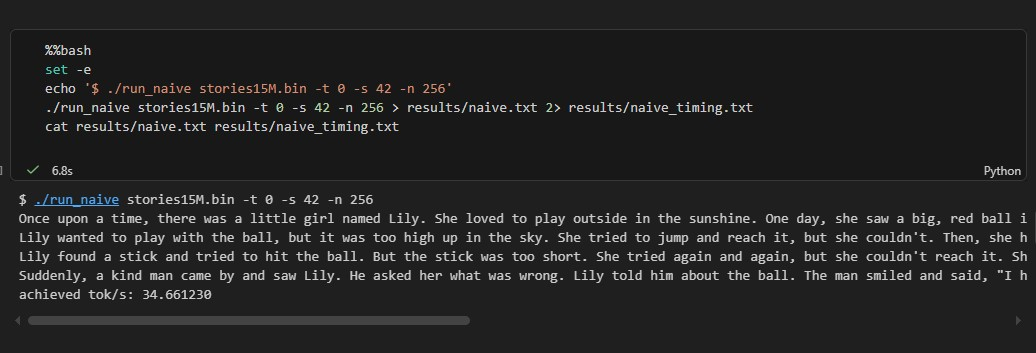
\includegraphics[width=\linewidth]{report_figures/49.jpg}
  \caption{Naive CUDA backend, matched workload (execution 49).}
\end{figure}

\begin{figure}[H]
  \centering
  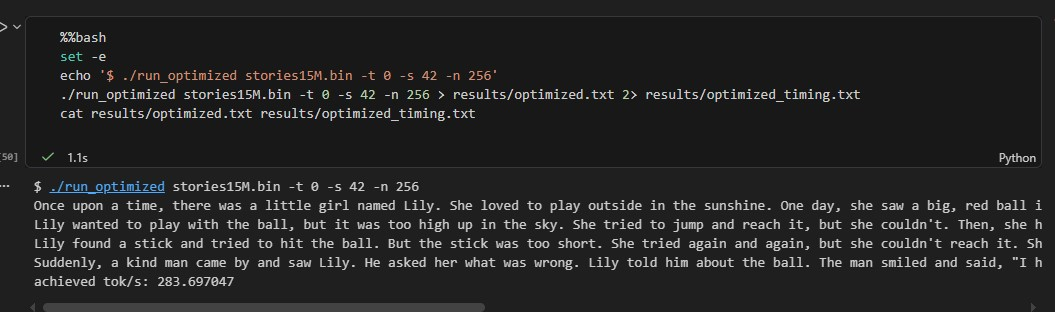
\includegraphics[width=\linewidth]{report_figures/50.jpg}
  \caption{Optimized CUDA backend, matched workload (execution 50).}
\end{figure}

\end{document}
